\section{Kurtosis}
Veri dağılımının sivrilik derecesini ölçen bir istatistiksel terimdir. Kurtosis, veri dağılımının kuyrukluluğunu ve ağırlıklı olarak merkezi değerlerin etrafında ne kadar veri noktası yoğunlaştığını ifade eder. Pozitif kurtosis değerleri, veri dağılımının sivrilen bir zirveye sahip olduğunu ve kuyrukların daha ağırlıklı olduğunu gösterirken, negatif kurtosis değerleri, veri dağılımının daha düz bir zirveye sahip olduğunu ve kuyrukların daha hafif olduğunu gösterir. 3 türdedir:

\begin{figure}[h]
    \centering
    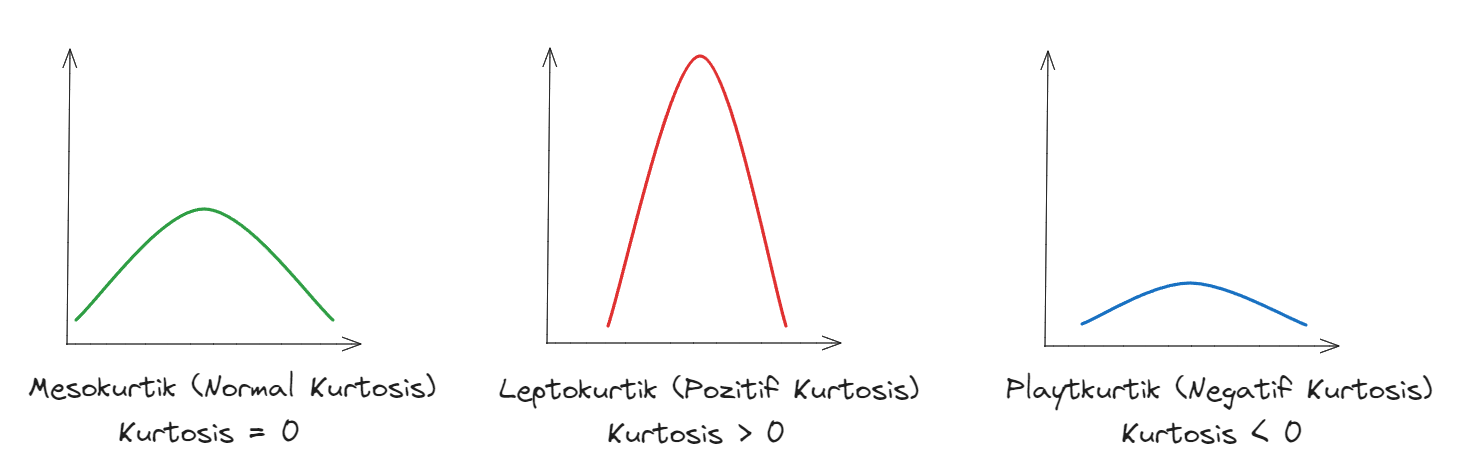
\includegraphics[width=1\textwidth]{images/kurtosis.png}
    \caption{Basıklık türleri.}
    \label{fig:enter-label}
\end{figure}

\begin{itemize}
    \item \textbf{Mesokurtik (Normal Kurtosis):} Normal dağılımdır. Kurtosis = 0.
    \item \textbf{Leptokurtik (Pozitif Kurtosis):} Normal dağılımdan daha sivri ve dar bir zirveye sahiptir. Kurtosis > 0.
    \item \textbf{Playtkurtik (Negatif Kurtosis):} Normal dağılıma göre daha düz bir zirveye sahiptir. Kurtosis < 0.
\end{itemize}

\newpage